\chapter{Datos y metodología}
\label{chapter:datos_metodologia}

\section{Datos: La Encuesta Financiera de las Familias}\label{section:datos}

Para este proyexto se van a utilizar los datos de la Encuesta Financiera de las Familias (EFF). La EFF es una encuesta oficial a hogares elaborada por el Banco de España y está incluida en el Plan Estadístico Nacional. Su primera edicion se realizó en el año 2002, y se ha producido de manera trienal hasta el año 2020. Desde entonces, se produce de manera bienal.

El objetivo de la EFF es recabar información sobre las condiciones financieras de los hogares residentes en España. Su cuestionario principal está compuesto por nueve secciones. Las secciones 1 y 6 recogen información sociodemográfica individualizada de todos los miembros del hogar y también información individualizada sobre la situación laboral y los ingresos de cada miembro del hogar mayor de 16 años. El resto de secciones recogen información detallada sobre los activos, deudas, gastos y uso de medios de pago del hogar en su conjunto, y contienen módulos específicos que recogen información individualizada de ciertos elementos patrimoniales si el hogar los posee, como propiedades inmobiliarias, negocios gestionados por cuenta propia o planes de pensiones. Los hogares formados por más miembros mayores de edad y que posean más elementos patrimoniales responderán a más preguntas. Por poner un ejemplo con números, en la EFF2017 a cada hogar se le plantearon entre 137 y 594 preguntas, siendo la mediana de 259 preguntas (\cite{effmethod2017}).

La EFF es la única fuente estadística que permite relacionar información sobre activos, deudas, ingresos y gastos de los hogares españoles. Esto permite analizar las decisiones de inversión y financiación de las familias y conocer su situación patrimonial, y gracias a ello tener un mayor conocimiento de la economía española y poder utilizarlo para hacer un diseño adecuado de politicas públicas. Por nombrar algunos ejemplos de estudios realizados con la EFF, se ha utilizado para cuantificar el ahorro adicional generado para los partícipes en planes de pensiones de empresa (\cite{gomez2022pensiones}), para caracterizar cómo afectó la pandemia del Covid-19 a la situación patrimonial de los trabajadores más afectados por dicha crisis (\cite{alvargonzalez2020pandemia} o para analizar las diferencias en aceptación y uso de tarjetas de crédito y banca online entre diferentes grupos de hogares desde el año 2002 (\cite{crespo2023bancaonline}).

El diseño de la muestra de la EFF tiene dos características importantes: un sobremuestreo de hogares ricos y un componente longitudinal o panel. El sobremuestreo de ricos\footnote{La muestra de la EFF es seleccionada por el Instituto Nacional de Estadística, en colaboración con la Agencia Tributaria, a partir de las declaraciones individuales más recientes en el Impuesto sobre el Patrimonio. Para una descripción más detallada del proceso, puede consultarse \cite{effmethod2017}.} garantiza poder analizar con suficiente precisión el comportamiento de los hogares de la parte alta de la distribución de riqueza. Este detalle es importante porque la distribución de la riqueza entre los hogares es asimétrica, por lo que sólo unos pocos hogares, especialmente los más ricos, son los que invierten en ciertos activos. Por otro lado, el compomente panel indica que se vuelve a entrevistar a hogares que participaron en ediciones anteriores. Esto permite monitorearles durante períodos de hasta diez años, y observar los cambios en las variables de interés de la encuesta. El número máximo de ediciones en las que un hogar puede participar en la EFF es de cuatro olas consecutivas. Si cesa su participación antes de completar sus cuatro ediciones, se descarta de la muestra y no vuelve a ser contactado en olas posteriores. Finalmente, para sustituir a los hogares descartados del panel rotatorio y mantener la representatividad de la muestra, en cada nueva ola de la EFF se añade una nueva muestra de refresco a la muestra panel.

Volviendo a los datos, en este proyecto se utiliza información que proviene tanto de las respuestas al cuestionario de la EFF, como del paradata recopilado durante la producción de los datos. En la figura 4.1. puede observarse un resumen de este proceso. La producción de la EFF se divide en dos grandes fases: Campo y Post-Campo. Durante el Campo se contacta con los hogares, se realizan las entrevistas personales, se procesan los datos y se realiza parte de la revisión de los mismos. En el Post-Campo se termina el proceso de revisión, se evalúa el grado de no-respuesta de los datos de cada hogar para eliminar las entrevistas con poco contenido informativo, y se procede a la imputación de la no-respuesta. Tras este último proceso, se obtienen los datos finales.

\begin{figure}[h]
	\centering
	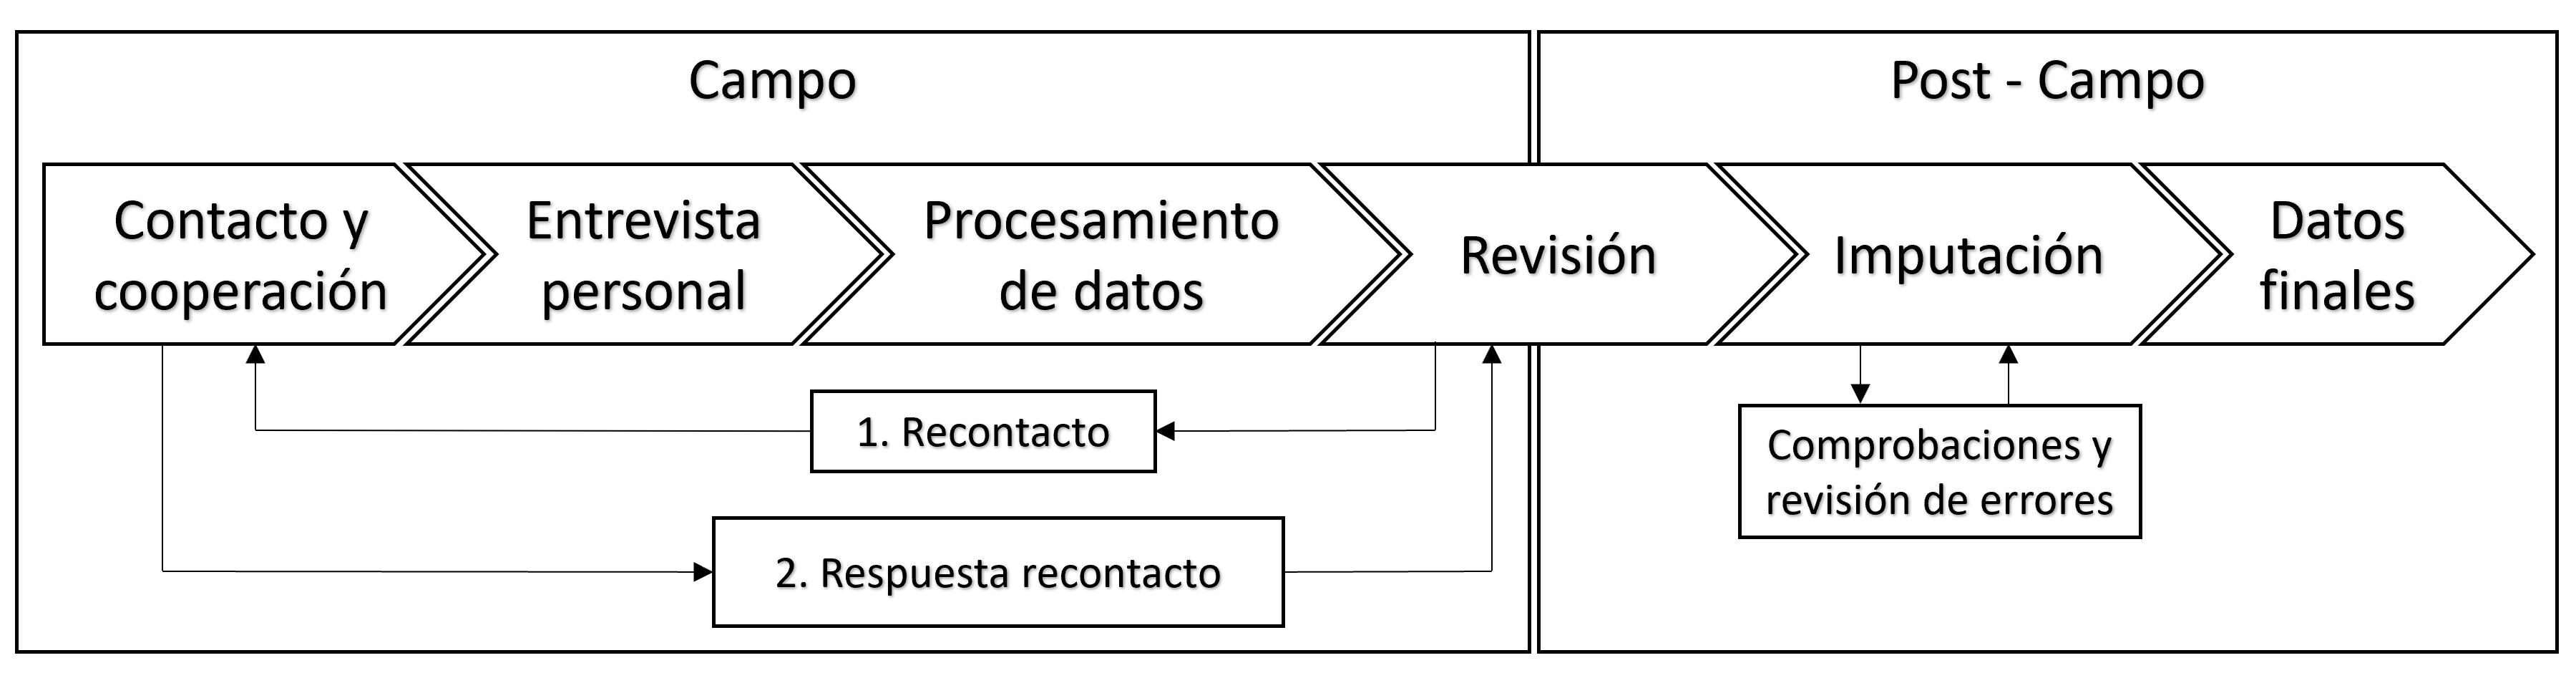
\includegraphics[width=1\textwidth]{figs/fases_creacion_datos_eff.png}
	\caption{Fases de la creación de datos de la EFF}
	\label{fig:eff_phases}
\end{figure}

A continuación se hace una breve descripción de los aspectos más relevantes de las subfases y que son importantes para la selección de variables para este estudio.

\begin{itemize}
    \item \textbf{Contacto y cooperación:} Los entrevistadores realizan visitas personales a los hogares en sus domicilios. Esto puede requerir varios intentos, ya que es necesario que algún miembro del hogar esté físicamente en su hogar cuando tenga lugar la visita presencial. La información sobre cada intento (fecha y hora, resultado...) se recoge en un ordenador. Antes de establecer el contacto, los entrevistadores rellenan un cuestionario que recoge información sobre las características del barrio y del edificio en el que vive el hogar.
    \item \textbf{Entrevista personal:} Se realiza una entrevista personal a la persona con más conocimiento de las finanzas del hogar, que se denomina Persona de Referencia o PR. La PR puede ser miembro del hogar, o un representante del mismo, demoninado proxy, siempre y cuando sea la persona con mayor conocimiento de las finanzas del hogar. También pueden participar otros miembros del hogar. Antes de empezar la entrevista, se pide a la PR su consentimiento para que algunas partes de la misma puedan ser grabadas en audio por motivos de calidad de los datos. La entrevista puede realizarse aunque no haya grabación. Los entrevistadores recogen las respuestas en un ordenador o una tablet (CAPI), y también pueden anotar en comentarios de texto todos los detalles que consideren importantes para la revisión. La PR puede decidir no contestar a ciertas preguntas. Su valor se asignará como missing, y se imputará más adelante. Las cantidades monetarias pueden responderse en valor puntual, o dentro de un rango de valores. Tras la entrevista, y sin la presencia de los hogares, los entrevistadores rellenan un cuestionario con información sobre el desarrollo de la entrevista, en el que por ejemplo se recoge el nivel de comprensión de la PR a las preguntas, el nivel de interés mostrado por la PR o cuántas personas han participado en la entrevista.
    \item \textbf{Procesamiento de datos:} Los ordenadores y servidores de la empresa de campo procesan los datos recogidos durante el contacto con los hogares y durante las entrevistas. Se crean tres ficheros, uno con las respuestas al cuestionario, uno con la información de los contactos con cada hogar, y finalmente uno con la información del paradata recogido por el ordenador durante la entrevista\footnote{También se crea un fichero con los comentarios de texto recogidos por los entrevistadores durante la entrevista, pero no se ha podido incluir en este estudio por falta de tiempo.}.
    \item \textbf{Revisión:} Un equipo de personas revisa individualmente todas las entrevistas y corrige los errores que puedan detectarse. Si hay información relevante que se ha recogido erróneamente o se ha omitido, se contacta de nuevo con el hogar para corregirlo o recuperar esa información. Este recontacto se hace por teléfono. Toda la información sobre la revisión (cambios sobre variables, recontactos...) se recoge en una aplicación informática y puede ser exportada en ficheros de diversos formatos (csv, excel...).
    \item \textbf{Imputación:} Se analiza la proporción de preguntas sin responder dentro de cada entrevista (no-respuesta), y se eliminan las que no superen ciertos umbrales de calidad. Todas las variables que contienen no-respuesta se imputan mediante técnicas de imputación múltiple\footnote{Los métodos de imputación múltiple utilizados en la EFF pueden consultarse en \cite{barcelo2006imputation}.}. Se crean 5 ficheros con datos imputados.
\end{itemize}

Con respecto a los procedimientos de Contacto y Entrevista personal, es necesario mencionar que algunos elementos tuvieron que modificarse durante la EFF2020, ya que el campo tuvo lugar entre noviembre de 2020 y junio de 2021, y se vió afectado por la pandemia del Covid-19. Durante esa ola, los entrevistadores siguieron visitando personalmente a los hogares para conseguir su colaboración\footnote{Durante el principio del campo, algunos hogares panel fueron contactados sólo por teléfono, pero a las pocas semanas se decidió establecer la visita personal como el procedimiento estándar.}, pero siempre respetando las medidas de distanciamiento social. Las entrevistas se realizaron de manera telefónica asistida por una tablet (CATI). El resto de procedimientos se mantuvieron como en otras ediciones.

Para la elaboración de este proyecto se utiliza la información recopilada durante las olas de la EFF2017, EFF2020 y EFF2022 \footnote{En el momento de escribir este documento, la EFF2022 se encontraba en pleno proceso de imputación, por lo que el equipo del Banco de España ya conocía los resultados de participación de esa ola y era posible utilizarlos para este proyecto.}. Estas ediciones son las únicas que cuentan con la información más detallada de paradata y de las características de los entrevistadores. En ediciones anteriores esta información o no está disponible, o contiene errores de medida que no son fácilmente corregibles. A pesar de esto, es posible identificar en cuántas ediciones ha participado cada hogar, por lo que es posible utilizar información que se remonta hasta la edición de la EFF2011. Los ficheros de datos que se han utilizado durante este proyecto son:

\begin{itemize}
    \item \textbf{Fichero de trabajo:} Registro de hogares con entrevistas válidas. Contiene la información de las respuestas de los hogares, incluyendo las correcciones y ediciones de la revisión. Se indican los datos que deben ser imputados. También incluye variables auxiliares generadas para el proceso de imputación (características del hogar, de los miembros, del municipio...) y contadores de no respuesta de cada entrevista. Es el fichero que se utiliza para imputar.
    \item \textbf{Fichero de datos imputados:} Registro de hogares que contiene las respuestas al cuestionario después de haber imputado los datos con no-respuesta de los hogares. Por simplicidad, sólo utilizaremos uno de los conjuntos de datos de la imputación multiple. Sólo contiene variables imputadas e indicadores de las características del hogar.
    \item \textbf{Fichero de contactos:} Registo de hogares contactados durante una ola de la EFF. Contiene información sobre el número de intentos de contacto con cada hogar, la fecha en que se produjo, el resultado de cada uno de ellos (aplazamientos, rechazos...) y las respuestas al cuestionario de vecindario rellenado por los entrevistadores.
    \item \textbf{Fichero de revisión:} Registro de hogares e incidencias que contiene información sobre el proceso de revisión y los recontactos. Para cada hogar hay varios registros. Uno contiene información general sobre el proceso de revisión (por ejemplo, si se ha realizado un recontacto), y el resto de registros son incidencias en los datos que se detectado (por ejemplo, si se ha omitido una propiedad inmobiliaria, se abrirá un registro indicando esa incidencia y cómo se ha solucionado).
    \item \textbf{Censo de entrevistadores:} Registro de entrevistadores que contiene la información disponible sobre los entrevistadores que han participado desde la EFF2014 a la EFF2022.
    \item \textbf{Fichero de paradata:} Registro con información sobre las pantallas del software CAPI que se utilizó durante la entrevista. Para cada hogar, contiene información detallada de la interacción del entrevistador con el ordenador durante la entrevista. En concreto, contiene el flujo de pantallas que se visualizaron en el ordenador en cada entrevista, y para cada pantalla se registra la fecha y hora en la que entró, si volvió a la pantalla anterior, o el tiempo que estuvo en cada pantalla.
\end{itemize}

\section{Metodología}

Tomando como referencia las estrategias de investigación propuestas en \cite{oates2022researching}, en este proyecto se presenta un 'Caso de estudio'. Se busca tener un conocimiento profundo sobre la participación de los hogares panel en el caso específico de la EFF, y buscar un modelo para predecirla.

La metodología de este proyecto se fundamenta en cuatro pilares. En primer lugar, en la recopilación de los datos de las entrevistas y los entrevistadores que participaron en las olas EFF2017, EFF2020 y EFF2022. El segundo pilar es la realización de un análisis descriptivo de un conjunto de variables con potencial para explicar la Attrition. En tercer lugar, en el entrenamiento de varios modelos basados en métodos de machine learning con datos de la EFF2017 y la EFF2020, y evaluar su rendimiento para predecir la participación de los hogares panel en la EFF2022. Para este ejercicio se adapta la implementación hecha en \cite{beste2023case} al caso de la EFF. Finalmente, se realiza una valoración de los resultados obtenidos y qué pasos podrían darse en el futuro para seguir desarrollando este proyecto.

El resto de esta sección se divide en tres apartados. Es primer lugar se da una breve descripción del proceso de recopilación de los datos. En el siguiente apartado se define la variable dependiente $Attrition$ y también las variables que se van a utilizar como predictores de los modelos. Finalmente, se cierra este capítulo con la descripción de la estrategia de entrenamiento y validación de los modelos.

\subsection*{Recopilación de datos}

Como acabamos de comprobar, en la EFF hay, por un lado, información sobre las entrevistas a los hogares repartida en varios ficheros para cada ola en la que han participado; y por otro lado, información sobre los entrevistadores que han colaborado en la EFF recogidas en un censo. La unidad de análisis de este estudio son hogares que ya han participado al menos una vez en alguna edición de la EFF, y que son elegibles para ser entrevistados en la siguiente edición. Por tanto, para cada ola se selecciona sólo a los hogares que han participado como máximo en tres ediciones, ya que los que han participado en la cuarta son eliminados de la muestra de cara a la siguiente edición. Los datos de una ola en concreto se utilizan como variables explicativas en los modelos, y como variable objetivo se extraerá el estatus de participación de ese mismo hogar del fichero de contactos de la ola siguiente. La vinculación de la información entre ambas ediciones se realiza a través de un identificador común que tienen los hogares en los ficheros de datos de ambas olas.

Por otro lado, la vinculación con la información del censo de entrevistadores se realiza a través de un identificador único que tiene cada entrevistador y que permanece inalterable a lo largo de las olas. Para cada hogar se conoce el identificador de la persona que realizó la entrevista en cada una de las olas en las que participó.

%\vspace{-5pt}

\subsection*{Variable Attrition y predictores}

El objetivo del estudio es encontrar un modelo para predecir si un hogar que ha participado en la ola $t$ de la EFF no volverá a participar en la siguiente ola $t+1$. Para ello, se define la variable \textit{Attrition} como una variable dicotómica que toma valor 0 si el hogar vuelve a participar, y valor 1 si no vuelve a participar:

\begin{equation}
Attrition =
  \begin{cases}
    0       & \quad \text{el hogar participa en la ola $t+1$} \\
    1  & \quad \text{el hogar no participa en la ola $t+1$}
  \end{cases}
\end{equation}

En el cuadro \ref{table:attrition} puede observarse que, en las olas de 2020 y 2022, la mayoría de los hogares panel volvieron a participar. Aunque parezca que sólo un ligero desbalance entre las observaciones de cada clase de Attrition, durante los primeros entrenamientos y evaluaciones de los modelos se comprobó que las predicciones se asignaban masivamente a la clase mayoritaria ($Attrition=0$). Para evitar esto, y dado el tamaño limitado de la muestra, previo al entrenamiento se procede al balanceo de la clase Attrition realizando un sobre-muestreo de dicha clase usando el algoritmo SMOTE (Syntetic Monirity Over-sampling Technique, \cite{chawla2002smote}).

\begin{table}[ht]
\centering{}
\begin{tabular}{lcc}
\textbf{Attrition}           & \textbf{EFF2020} & \textbf{EFF2022} \\ \hline
Participa (attrition = 0)    & 3830             & 3974             \\
No participa (attrition = 1) & 2107             & 1531             \\ \hline
\end{tabular}
\caption{\textit{Distribución de Attrition en EFF2020 y EFF2022}}
\label{table:attrition}
\end{table}

En el otro lado de un modelo de predicción se encuentran las variables que se eligen como predictores. Por definición, estas variables deben contener información conocida y observable antes de que se producza el fenómeno que se quiere predecir. En ese sentido, para predecir \textit{Attrition} en $t+1$ se utilizan como predictores variables que se corresponden con la ola anterior, la ola $t$. La selección de estas variables se ha inspirado en la realizada por \cite{beste2023case} y \cite{kern2021predicting}, y adicionalmente se han incluido otras variables de interés para la EFF, como por ejemplo si un hogar se ha recontactado durante la revisión o si la entrevista se realizó con un proxy. La selección final de 57 variables explicativas utilizadas en este estudio puede consultarse en el cuadro \ref{table:vars}.

\begin{table}[ht]
    \centering
    \begin{tabular}{|l|p{10cm}|}
    \hline
        \textbf{Fuente de información} & \textbf{Variables} \\ \hline
        Características del hogar & Número de adultos con empleo, Número de adultos jubilados, Propietario vivienda principal, Tamaño del hogar, Tiene otras propiedades, Tiene joyas, Posee negocios, Posee cuentas para pagos, Posee acciones que cotizan, Posee acciones que no cotizan, Posee renta fija, Posee fondos de inversión, Posee cuentas para no pagos, Posee planes de pensiones, Les deben dinero, Poseen vehículos, Percentil de renta, Percentil de riqueza Bruta, Pareja vive en el hogar, Poseen otros activos financieros, Tienen deuda, Tienen ingresos de activos, Hijos viven en el hogar, Nivel de satisfacción con la vida \\ \hline
        Características PR & Nivel de satisfacción con la vida, Es panel, Nivel educativo, Estado de salud, Edad, Estado Civil - Casada, Estado Civil - Viuda, Sexo, Situación laboral - Asalariado, Situación laboral - Jubilado, Situación laboral - Inactivo \\ \hline
        Valoraciones FI & Recelo tras la entrevista, Edificio Unifamiliar, Barreras - portero automático, Barreras - Sin barreras, Entendimiento de las preguntas por parte de PR, Interés de PR, Razones colaborar - Interesado en estos estudios, Razones para colaborar - Lo lleva el BdE, Razones para colaborar - Relevancia de la encuesta, Razones - Favor al entrevistador, Razones - Dar su opinión, Razones - Otras \\ \hline
        Paradata & PR consiente grabar la entrevista, Hogar recontactado, Número de olas en las que se ha participado, Tamaño del municipio, Entrevista con proxy, Número de miembros del hogar que participan en la entrevista, Porcentaje de preguntas monetarias respondidas en valor puntual, Porcentaje de preguntas monetarias respondidas (incluye intervalos), Número de variables con valores missing, Duración de la entrevista en segundos \\ \hline
    \end{tabular}
    \caption{Selección de variables para entrenar los modelos de predicción}
    \label{table:vars}
\end{table}

\subsection*{Entrenamiento, validación y test de modelos de machine learning}

La estrategia de entrenamiento y validación utilizada en este proyecto se inspira en la implementada en \cite{beste2023case}. Se entrenan cuatro modelos de predicción basados en algoritmos de machine learning, y se compara su rendimiento con un modelo de referencia que se utiliza tradicionalmente para analizar Panel Attrition. Este modelo base es una Regresión Logística o Logit de efectos primarios (sin interacciones entre variables y sin especificaciones no lineales). Los modelos de machine learning que se entrenan y evalúan son un árbol de decisión (CART), un Random Forest (RF), un eXtreme Gradient Boosting (XGBOOST) y un Naive Bayes (NB). La elección de estos modelos se fundamenta, por un lado, en los buenos resultados que han mostrado para predecir panel attrition en otras encuestas para hogares (\cite{kern2019tree}, \cite{kern2021predicting}, \cite{beste2023case}) y, por otro lado, en que estos modelos son fácilmente interpretables en comparación con otros algoritmos de machine learning, como pueden ser las máquinas de soporte venctorial(SVM) o las redes neuronales. Esto facilita que sean utilizados para diseños adaptativos y reactivos.

Con respecto al proceso de entrenamiento y evaluación, a la hora de elegir los conjuntos de entrenamiento, validación y test, se tiene en cuenta el uso que se querría dar al algoritmo en la práctica. El objetivo es predecir qué hogares tienen más probabilidad de abandonar el estudio en la ola siguiente antes de que ésta tenga lugar. Por un lado,Eso implica establecer un criterio de separación temporal entre los conjuntos de entrenamiento y test, y asegurar que en los predictores de los modelos sólo se incluye información conocida ex-ante. En ese sentido, siguiendo la idea propuesta en \cite{beste2023case}, utilizaremos exclusivamente información disponible en una ola concreta para predecir el resultado de la participación en la siguiente. Por esa razón, para el entrenamiento y la validación de los modelos, se utiliza la información recopilada en la EFF2017 para predecir la participación en EFF2020, y para el ejercicio del test se utiliza la información recopilada en la EFF2020 para predecir la participación en la EFF2022.

Para el tuning de los hiperparámetros de los modelos, se sigue una estrategia de k-fold cross-validation para los conjuntos de entrenamiento y validación, con k=5. Con respecto a los valores específicos de los hiperparámetros, como no existe certeza sobre cuáles son los valores más adecuados, se considera un rango bastante amplio para cada hiperparámetro de todos los algoritmos. Para los modelos Logit y CART se utiliza un algoritmo de búsqueda de red (grid search) para probar cada combinación de hiperparámetros. Con respecto a los algoritmos RF y XGBOOST, dados los elevados tiempos y costes de ejecución de cada uno, se utiliza un algoritmo de búsqueda aleatoria (random search) con 2500 iteraciones. Aunque no se prueben todos los valores de los hiperparámetros, se ha comprobado que la búsqueda aleatoria es una alternativa válida en contextos de alta dimensionalidad de hiperparámetros (\cite{bergstra2012random}). Finalmente, a la hora de seleccionar las mejores combinaciones de modelos, la métrica que se busca maximizar es la ROC AUC.